\section{Multi-arm Bandits}

RL evaluates the actions taken rather than instructs correct actions like other forms of learning.

\subsection{An n-Armed Bandit Problem}
\textbf{The problem}:\\
\begin{itemize}
\item You are faced repeatedly with a choice of \textit{n} actions.
\item After each choice, you receive a reward from a stationary probability distribution.
\item Objective is to maximise total reward over some time period, say 100 time steps.
\item Named after of slot machine (one-armed bandit problem), but \textit{n} levers instead of 1.
\item Each action has an expected or mean reward based on it's prob distribution. We shall call that the \textit{value} of the action. We do not know these values with certainty.
\item Because of this uncertainty, there is always an exploration vs exploitation problem. We always have one action that we deem to be most valuable at any instant, but it is highly likely, at least initially, that there are actions we are yet to explore that are more valuable.
\end{itemize}

\subsection{Action-Value Methods}
\textbf{The estimated action value}
\begin{equation} \label{eq: estimated value}
	Q_t(a) = \frac{R_1+R_2+\cdots+R_{N_t(a)}}{N_t(a)}
\end{equation}

The true value (mean reward) of an action is \(q\), but the estimated value at the \textit{t}th time-step is Q(a), given by Equation \ref{eq: estimated value} (our estimate after \textit{N} selections of an action yielding \textit{N} rewards).\\

\noindent \textbf{The greedy action selection method:}
\begin{equation} \label{eq: argmax}
A_t =\argmax_a Q_t(a)
\end{equation}

\begin{itemize}
	\item Simplest action selection rule is to select the action with the highest estimated value.
	\item Argmax a means the value of \(a\) for which \(Q_t\) is maximised.
	\item \(\epsilon\)-greedy methods are where the agent selects the greedy option most of the time, and selects a random action with probability \(\epsilon\).
	\item Three algorithms are tried: one with \(e\)=0 (pure greedy), one with \(e\)=0.01 and another with \(e\)=0.1
\end{itemize}

\begin{figure}[h!]
	\centering
	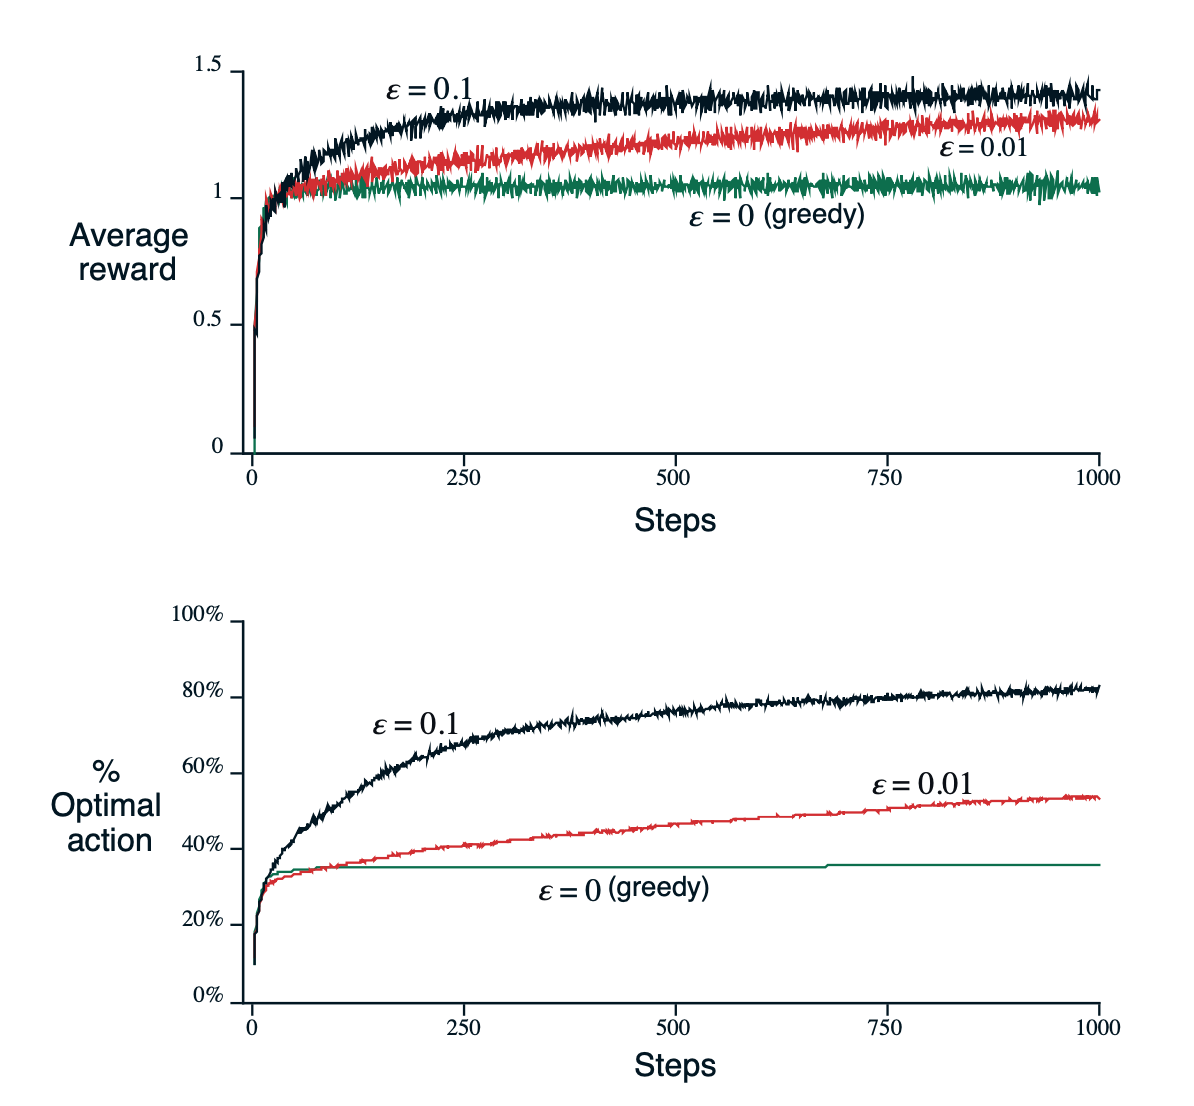
\includegraphics[width=\textwidth]{/chapter2_1}
	\caption{tbc}
	\label{fig:chapter2_1}
\end{figure}

\begin{itemize}
	\item Greedy method gets stuck performing sub-optimal actions.
	\item \(e\)=0.1 explores more and usually finds the optimal action earlier, but never selects it more that 91\% of the time.
	\item \(e\)=0.01 method improves more slowly, but eventually performs better than the e=0.1 method on both performance measures.
	\item It is possible to reduce \(e\) over time to try to get the best of both high and low values.
\end{itemize}

\subsection{Incremental Implementation}
The sample-average technique used to estimate action-values above has a problem: memory and computation requirements grow over time. This isn't necessary, we can devise an incremental solution instead:

\begin{align}
	Q_{k+1} &= \frac{1}{k}\sum_{i}^{k}R_i \nonumber \\
	&= \frac{1}{k} \left( R_k + \sum_{i=1}^{k-1} R_i \right) \nonumber \\
	&= \vdots \\
	&= Q_k + \frac{1}{k} \left[R_k - Q_k\right] \\
\end{align}

We are updating our estimate of \(Q_{k+1}\) by adding the discounted error between the reward just received and our estimate for that reward \(Q_k\).

\begin{equation}
NewEstimate \leftarrow OldEstimate + StepSize \left[Target - OldEstimate \right]
\end{equation}

\(\alpha\) is used to denote the stepsize (\(\frac{1}{k}\)) in the rest of this book.

\subsection{Tracking a Nonstationary Problem}
The averaging methods discussed above do not work if the bandit is changing over time. In such cases it makes sense to weight recent rewards higher than long-past ones. The popular way of doing this is by using a constant step-size parameter.

\begin{equation}
	Q_{k+1} = Q_k +\alpha \left[R_k - Q_k\right]
\end{equation}

where the step-size parameter \(\alpha \in (0,1]\) is constant. This results in \(Q_{k+1}\) being a weighted average of the past rewards and the initial estimate \(Q_1\):

\begin{align}
Q_{k+1} &= Q_k +\alpha \left[R_k - Q_k\right] \nonumber \\
&= \alpha R_k + (1 - \alpha)Q_k \nonumber \\
&= \alpha R_k + (1 - \alpha)[\alpha R_{k-1} + (1 - \alpha)Q_{k-1}] \nonumber \\
&= \alpha R_k + (1 - \alpha)\alpha R_{k-1} + (1 - \alpha)^2 Q_{k-1}  \nonumber \\
&= \vdots \nonumber \\
&= (1-\alpha)^k Q_1 + \sum_{i}^{k} \alpha (1 - \alpha)^{k-i} R_i \\
\end{align}

\begin{itemize}
\item Because the weight given to each reward depends on how many rewards ago it was observed, we can see that more recent rewards are given more weight. Note the weights \(\alpha\) sum to 1 here, ensuring it is indeed a weighted average where more weight is allocated to recent rewards.
\item In fact, the weight given to each reward decays exponentially into the past. This sometimes called an \textit{exponential} or \textit{recency-weighted} average.
\end{itemize}

\subsection{Optimistic Initial Values}
\begin{itemize}
\item The methods discussed so far are dependent to some extent on the initial action-value estimate i.e. they are biased by their initial estimates.
\item For methods with constant \(\alpha\) this bias is permanent.
\item In effect, the initial estimates become a set of parameters for the model that must be picked by the user.
\item In the above problem, by setting initial values to +5 rather than 0 we encourage exploration, even in the greedy case. The agent will almost always be disappointed with it's samples because they are less than the initial estimate and so will explore elsewhere until the values converge.
\item The above method of exploration is called \textit{Optimistic Initial Values}.
\end{itemize}

\subsection{Upper-confidence-bound Action Selection}
\(\epsilon\)-greedy action selection forces the agent to explore new actions, but it does so indiscriminately. It would be better to select among non-greedy actions according to their potential for actually being optimal, taking into account both how close their estimates are to being maximal and the uncertainty in those estimates. One way to do this is to select actions as:

\begin{equation}
	A_t = \argmax_a \left[Q_t(a) + c\sqrt{\frac{\ln t}{N_t(a)}}\right]
\end{equation}

where c \(>\) 0 controls the degree of exploration.

\begin{itemize}
	\item The square root term is a measure of the uncertainity in our estimate. It is proportional to \(t\) i.e. how many timesteps have passed and inversely proportional to \(N_t(a)\) i.e. how many times that action has been visited. The more time has passed, and the less we have sampled an action, the higher our upper-confidence-bound.
	\item As the timesteps increases, the denominator dominates the numerator as the ln term flattens.
	\item Each time we select an action our uncertainty decreases because N is the denominator of this equation.
	\item UCB will often perform better than e-greedy methods
\end{itemize}

\begin{figure}[h!]
	\centering
	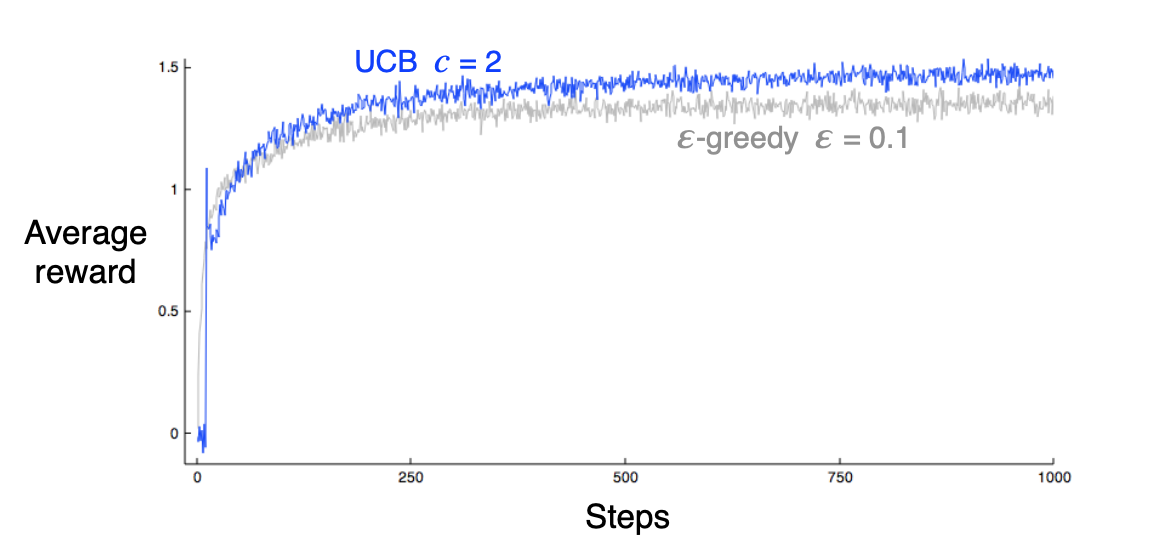
\includegraphics[width=\textwidth]{/chapter2_2}
	\caption{UCB performs better than \(e\)-greedy in the n-armed bandit problem}
	\label{fig:chapter2_2}
\end{figure}

\subsection{Associative Search (Contextual Bandits)}
\begin{itemize}
\item Thus far we have been discussing the stationary k-armed bandit problem, where the value of each arm is unknown but nonetheless remains stationary. Now, we consider a problem where the task could change from step to step, but the value distributions of the arms in each task remain the same. This is called contextual bandits, and in the toy example we are usually given a hint that the task has changed e.g. the slot machine changes colour for each task.
\item Now we want to learn the correct action to take in a particular setting, given the task colour observed. This is an intermediary between the stationary problem and the full reinforcement learning problem. See exercise 2.10 below.
\end{itemize}

\subsection{Key Takeaways}
\begin{itemize}
\item The value of an action can be summarised by \(Q_t(a)\), the sample average return from an action
\item When selecting an action, it is preferable to maintain exploration, rather than only selecting the action we believe to be most valuable at any given timestep, to ensure we continue to improve our best estimate of the optimal action. We do so using \(\epsilon\))-greedy policies.
\item If our problem is non-stationary, rather than taking a standard average of every return received after an action, we can take a weighted average that gives higher value to more recently acquired rewards. We call this an \textit{exponential} or \textit{recency-weighted} average.
\item Optimistic initial values encourage lots of early exploration as our returns always decrease our estimate of \(Q_t\) meaning the greedy actions remain exploratory. Only useful for stationary problems.
\item \(\epsilon\)-greedy policies can be adapted to give more value to actions that have been selected less-often, i.e. actions where we have higher uncertainty in their value, using \textit{upper-confidence-bound} action selection.
\item Lastly, each of these techniques have varied performance on the n-armed bandit test dependent on their parametrisation. Their performance is plotted in Figure \ref{fig:chapter2_4}.
\end{itemize}

\begin{figure}[h!]
	\centering
	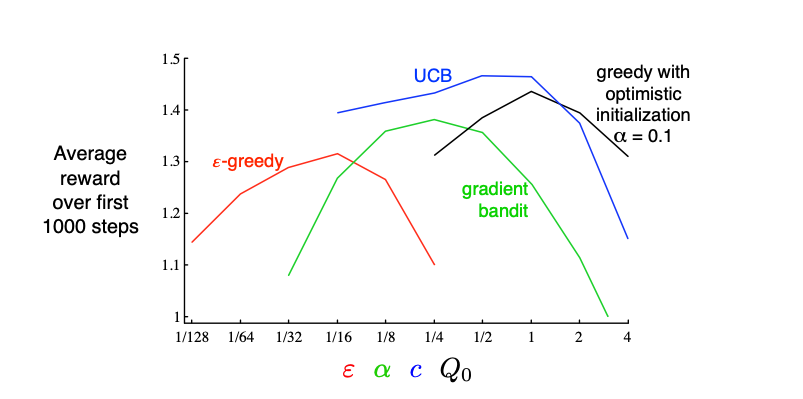
\includegraphics[width=\textwidth]{/chapter2_4}
	\caption{Performance of each of the bandit algorithms explored in this chapter}
	\label{fig:chapter2_4}
\end{figure}

\subsection{Exercises}
\subsubsection{Exercise 2.1}
\textbf{Q}\\
In \(e\)-greedy action selection, for the case of two actions and \(e\) = 0.5, what is the probability that the greedy action is selected?\\

\textbf{A}\\
\begin{itemize}
	\item Greedy action selected with \(p\) = 0.5
\end{itemize}

\subsubsection{Exercise 2.2}
\textbf{Q}\\
Bandit example Consider a k-armed bandit problem with k = 4 actions, denoted 1, 2, 3, and 4. Consider applying to this problem a bandit algorithm using \(e\)-greedy action selection, sample-average action-value estimates, and initial estimates of \(Q_1(a)\) = 0, for all \(a\). Suppose the initial sequence of actions and rewards is A1 = 1, R1 = 1, A2 = 2, R2 = 1, A3 = 2, R3 = 2, A4 = 2, R4 = 2, A5 = 3, R5 = 0. On some of these time steps the \(e\) case may have occurred, causing an action to be selected at random. On which time steps did this definitely occur? On which time steps could this possibly have occurred?\\

\textbf{A}
\begin{table}[]
	\begin{tabular}{lllllll}
		\hline
		Timestep & \(Q_1\) & \(Q_2\) & \(Q_3\) & \(Q_4\) & Greedy action at timestep & Action selected \\ \hline
		0        & 0    & 0    & 0    & 0    & -                         & \(A_1\)            \\ \hline
		1        & 1    & 0    & 0    & 0    & \(A_1\)                      & \(A_2\)            \\ \hline
		2        & 1    & 1    & 0    & 0    & \(A_1/A_2\)                 & \(A_2\)            \\ \hline
		3        & 1    & 1.5  & 0    & 0    & \(A_2\)                      & \(A_2\)            \\ \hline
		4        & 1    & 1.66 & 0    & 0    & \(A_2\)                      & \(A_5\)            \\ \hline
		5        & 1    & 1.66 & 0    & 0    & \(A_2\)                      & end             \\ \hline
	\end{tabular}
\end{table}
\begin{itemize}
	\item Action selection at timesteps 0, 1 and 4 are random as they are not reward maximising - see Table \ref{table: ex2.2}.
	\item Action selection at timestep 2 could be random as \(A_1\) is also reward maximising - see Table \ref{table: ex2.2}.
\end{itemize}

\subsubsection{Exercise 2.3}
\textbf{Q}\\
In the comparison shown in Figure \ref{fig:chapter2_2}, which method will perform best in the long run in terms of cumulative reward and probability of selecting the best action? How much better will it be? Express your answer quantitatively.\\

\textbf{A}\\
\begin{itemize}
	\item In the limit of \(t \rightarrow \infty\), both non-zero \(e\)-greedy policies will learn the optimal action abd value function \(q*\). The policy with \(e\) = 0.01 will select the optimal action 10x more regularly than the policy with \(e\) = 0.1.
\end{itemize}
\subsubsection{Exercise 2.4}
\textbf{Q}\\
If the step-size parameters, \(\alpha_n\), are not constant, then the estimate \(Q_n\) is a weighted average of previously received rewards with a weighting different from that given by (2.6). What is the weighting on each prior reward for the general case, analogous to (2.6), in terms of the sequence of step-size parameters?.\\

\textbf{A}
For a n-dependent \(\alpha\) we have:
\begin{align}
	Q_{n+1} &= Q_n +\alpha_n \left[R_n - Q_n\right] \nonumber \\
	&= \alpha_n R_n + (1-\alpha_n) Q_n\nonumber \\
	&= \alpha_n R_n + (1-\alpha_n) \left[Q_{n-1} + \alpha_{n-1} \left[R_{n-1} - Q_{n-1} \right]\right]\nonumber \\
	&= \alpha_n R_n + \alpha_{n-1} R_{n-1} - \alpha_n \alpha_{n-1} R_{n-1} + (1-\alpha_n)(1-\alpha_{n-1}) Q_{n-1} \nonumber \\
	&= \vdots \nonumber \\
	&= \sum_{i}^{n} \alpha_n R_n - R_{n-1} \prod_{i}^{n} \alpha_n + Q_{1} \prod_{i}^{n}(1-\alpha_n) \\
\end{align}

\subsubsection{Exercise 2.5}
\textbf{Q}\\
Design and conduct an experiment to demonstrate the difficulties that sample-average methods have for nonstationary problems. Use a modified version of the 10-armed testbed in which all the \(q_*(a)\) start out equal and then take independent random walks (say by adding a normally distributed increment with mean 0 and standard deviation 0.01 to all the \(q_*(a)\)  on each step). Prepare plots like Figure 2.2 for an action-value method using sample averages, incrementally computed, and another action-value method using a constant step-size parameter, \(\alpha\) = 0.1. Use \(\alpha\) = 0.1 and longer runs, say of 10,000 steps.\\

\textbf{A}\\
\ProgrammingExercise
\begin{figure}[h!]
	\centering
	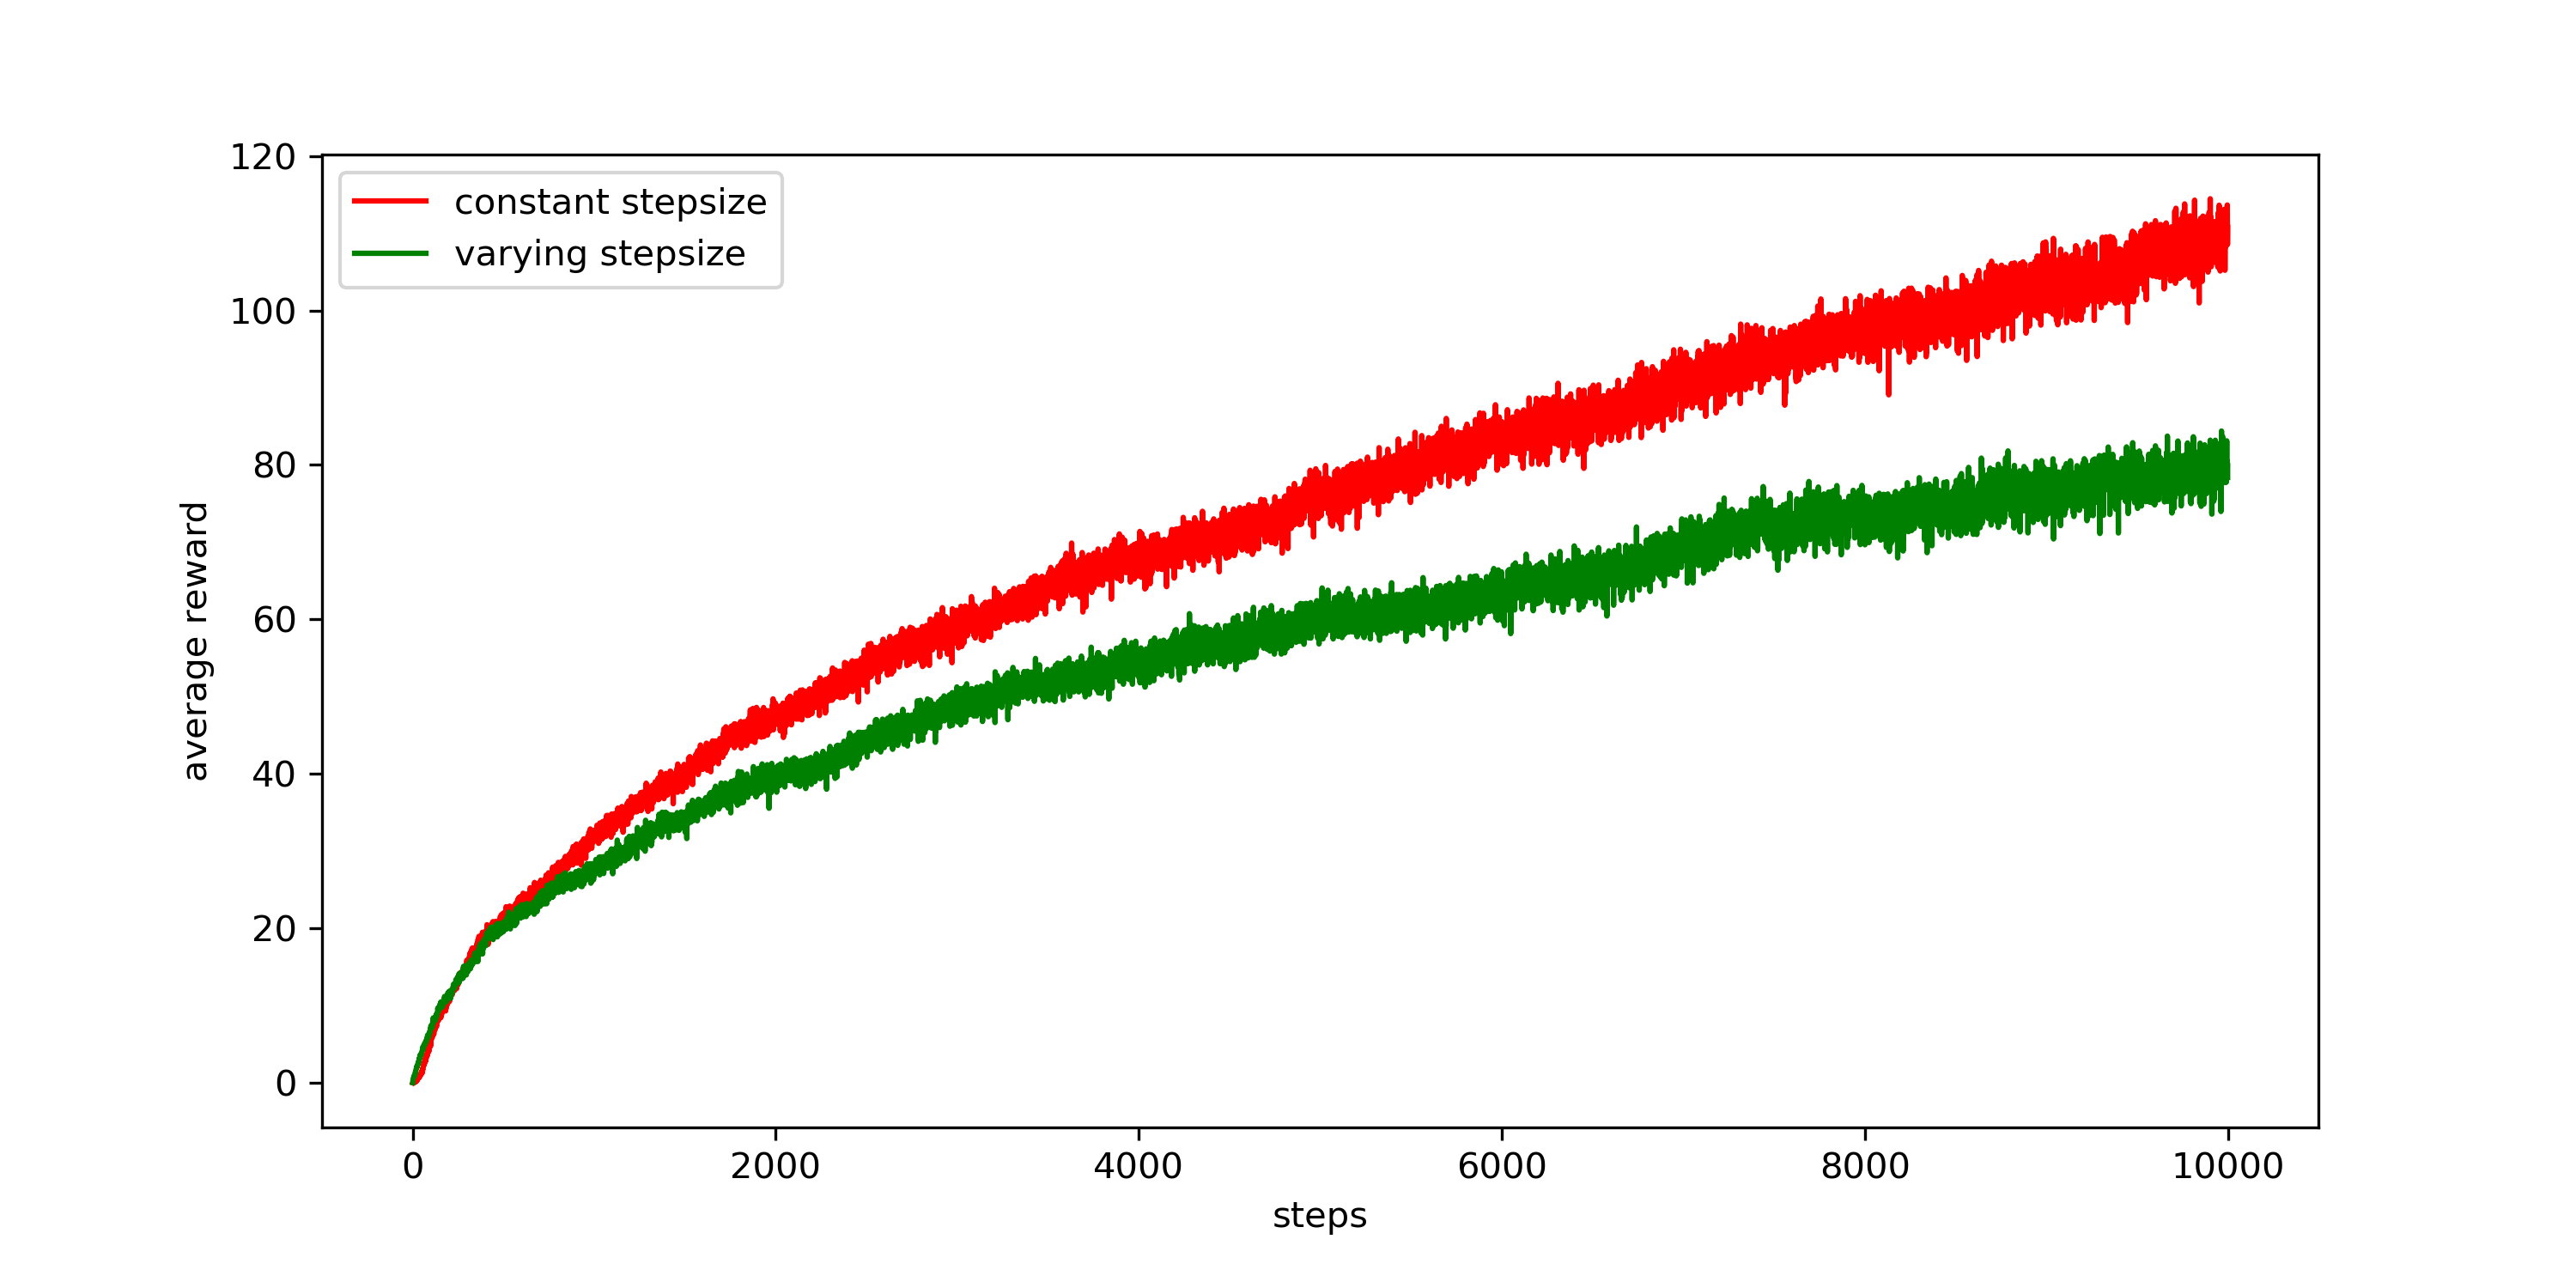
\includegraphics[width=\textwidth]{/ex2.5}
	\caption{Stationary versus varying stepsize \(alpha\) in a 10-armed bandit problem. We see that the constant stepsize parameter (exponential decay) performs better than the varying stepsize parameter as we place more weight on the recently observed (moving) values.}
	\label{fig:ex2.5}
\end{figure}

\subsubsection{Exercise 2.6}
\begin{figure}[h!]
	\centering
	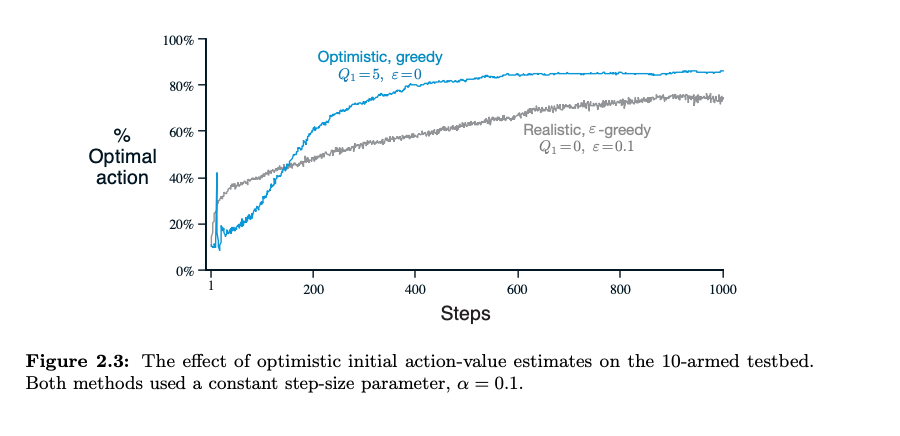
\includegraphics[width=\textwidth]{/chapter2_3}
	\caption{}
	\label{fig:chapter2_3}
\end{figure}
\noindent \textbf{Q}\\
\textit{Mysterious Spikes}: The results shown in Figure 2.3 should be quite reliable because they are averages over 2000 individual, randomly chosen 10-armed bandit tasks. Why, then, are there oscillations and spikes in the early part of the curve for the optimistic
method? In other words, what might make this method perform particularly better or worse, on average, on particular early steps?\\

\textbf{A}\\
The optimistic greedy policy with explore on every initial step as all value estimates are greater than their true value. It is possible, therefore, that it randomly selects the optimal action and then immediately forgets it in favour of yet-to-be-explored actions. This explains the spike at timestep \(\approx 10\).

\subsubsection{Exercise 2.7}
\textbf{Q}\\
Unbiased Constant-Step-Size Trick In most of this chapter we have used sample averages to estimate action values because sample averages do not produce the initial bias that constant step sizes do (see the analysis leading to (2.6)). However, sample averages are not a completely satisfactory solution because they may perform poorly on nonstationary problems. Is it possible to avoid the bias of constant step sizes while retaining their advantages on nonstationary problems? One way is to use a step size of
\begin{equation}
	\beta_n = \alpha / \bar{o_n}
\end{equation}

to process the \(n\)th reward for a particular action, where \(\alpha\) > 0 is a conventional constant step size, and ¯on is a trace of one that starts at 0:
\begin{equation}
	\bar{o_n} = \bar{o_{n-1}} + \alpha(1 - \bar{o_{n-1}}), for n > 0 and \bar{o_0} = 0.
\end{equation}

Carry out an analysis like that in (2.6) to show that Qn is an exponential recency-weighted
average without initial bias.\\

\textbf{A}\\
If we recall our answer for Exercise 2.4 for varying stepsize, we see that \(Q_1\) is weighted by \(w = \prod_{i=1}^{\infty} (1 - \alpha_i)\). When \(i\) = 1, \(\beta_n\) = \(\alpha\), thus \(w \rightarrow 0 \forall i\) and \(Q_1\) no longer affects our estimate of \(Q_{n+1}\).

\subsubsection{Exercise 2.8}
\textbf{Q}\\
\textit{UCB Spikes} In Figure \ref{fig:chapter2_2} the UCB algorithm shows a distinct spike in performance on the 11th step. Why is this? Note that for your answer to be fully satisfactory it must explain both why the reward increases on the 11th step and why it decreases on the subsequent steps. Hint: If c = 1, then the spike is less prominent.\\

\textbf{A}\\
After 10 timesteps the UCB algorithm has explored all 10 actions as, until they are selected, their upper confidence bound is infinite (as \(N_t(a)\) = 0) as so it guarenteed to be selected once in the first 10 actions. At this point the agent has one sample to assess the expected value of each arm and the same confidence/uncertainty in each action. With c < 0 it is likely to pick the action with highest return from first sample, which will likely give it an similarly large reward, creating the spike. Now, the upper confidence bound for that action will decrease and the agent will select another, less valuable action, causing the decrease in performance at the next timestep.
\subsubsection{Exercise 2.9}
\textbf{Q}\\
Show that in the case of two actions, the soft-max distribution is the same as that given by the logistic, or sigmoid, function often used in statistics and artificial neural networks.\\

\textbf{A}\\
Soft-max distribution is defined as:
\begin{equation}
	Pr{A_t = a} \approx \frac{e^{H_t(a)}}{\sum_{b=1}^{k} e^{H_t(b)}} \approx \pi_t(a)
\end{equation}

For two actions \(1\) and \(2\) this becomes:
%\begin{equation}
%Pr{A_t = 1} = \frac{e^{H_t(1)}}{e^{H_t(1) + e^{H_t(2)}} \nonumber \\
%= \frac{e^{H_t(1)}}{e^{H_t(1)}(1 + \frac{e^{H_t(2)}}{e^{H_t(1)}}} \nonumber \\
%= \frac{1}{e^{H_t(1)}(1 + e^{-x}} \nonumber\\
%\end{equation}
%i.e. the sigmoid function with x = \(H_t(1) - H_t(2)\).

\subsubsection{Exercise 2.10}
\textbf{Q}\\
Suppose you face a 2-armed bandit task whose true action values change randomly from time step to time step. Specifically, suppose that, for any time step, the true values of actions 1 and 2 are respectively 10 and 20 with probability 0.5 (case A), and 90 and 80 with probability 0.5 (case B). If you are not able to tell which case you face at any step, what is the best expected reward you can achieve and how should you behave to achieve it? Now suppose that on each step you are told whether you are facing case A or case B (although you still don’t know the true action values). This is an associative search task. What is the best expected reward you can achieve in this task, and how should you behave to achieve it?\\

\textbf{A}\\
Part 1): If we do not know whether we are in task A or B we could decide pick the same action each time to maximise expected reward. Selecting either action 1 or action 2 every time would provide an expected reward of 50. Picking actions randomly would also provide an expected reward of 50 in this example.
Part 2): If we know we are in task A or B we can learn the optimal action for each (A(a) = 2 and B(a) = 1). Doing so would provide us a higher expected reward than the non-contextual case of 55.